\section{Malware Classification}
\label{sec:ssdeep}

ssdeep~\cite{ssdeep} is a program to compute fuzzy hashes. 
Similarity between calculated hash strings can serve as an estimation for similarity between the two original files. 
ssdeep hash strings are also provided for each submitted file with other metadata fields by \vt. 
In this section, we explore the feasibility to build malware classifier and detector based on ssdeep similarity. 

Malware detectors mainly rely on signatures manually extracted by security researchers. 
ssdeep only takes static binary executable as inputs. 
If we can build malware detector based on ssdeep similarity, 
We can reduce or even eliminate manual efforts in malware detection. 


\subsection{Data Collection}

\begin{table*}
  \centering
  \scriptsize
  {
  \begin{tabular}{clccc}
    \toprule
{\bf Index} & {\bf Microsoft Tag} & {\bf \# of Malwares} & {\bf \% of Tailing}  & {\bf \% of Distinct}\\
\midrule                                                                                                                                                                                                                                           
1  &  SoftwareBundler:Win32/Penzievs 	& 49380	     & 3.51\%  & 99.98\%\\
2  &  Adware:Win32/Hotbar               & 132161   & 1.88\%  & 99.98\%\\
3  &  TrojanDropper:Win32/Lamechi!rfn	& 39205	     & 0.01\%  & 6.13\%\\
4  &  Virus:Win32/Nabucur.D	            & 1190132  & 99.95\% & 100.00\%\\
5  &  Virus:Win32/Virut.BO	            & 84600	   & 21.84\% & 99.95\% \\
6  &  Worm:Win32/Mydoom.L@mm	        & 76259	     & 0\%     & 99.44\%\\
7  &  Virus:Win32/Ramnit.I              & 412052   & 3.07\%  & 96.76\%\\
8  &  Trojan:Win32/Dorv.A               & 54324    & 2.80\%  & 80.53\%\\
9  &  Trojan:Win32/Dynamer!ac           & 145402   & 65.17\% & 99.20\%\\
10 &  Virus:Win32/Ramnit.A              & 181524   & 26.79\% & 99.82\%\\   

\bottomrule
   \end{tabular}
   }
   \mycaption{tab:benchmark}{Benchmark Information.}
{\footnotesize{(Information for malwares used in our clustering and classification experiments. \# of Malwares: \# of distinct malwares we collected in each sampled malware group from 05/07/2016 to 09/06/2016. \% of Tailing: \% of tailing examples in each group. \% of Distinct: number of distinct ssdeep hash strings divided by group size.)}}
  %\nocaptionrule
  %\mycaption{tab:benchmark}{Malware Data Set.}
  %\footnotesize{(Information for malwares used in our clustering and classification experiments. \# of Malwares: \# of distinct malwares we collected in each sampled malware group from 05/07/2016 to 09/06/2016. \% of Tailing: \% of tailing examples for each group in the sampled 10000 malwares.)}
 %}
\end{table*}




Microsoft has a good reputation in detecting PE malwares~\cite{SongAPsys2016}.
For each detected malware, Microsoft assigns it a tag, which contains type, platform, family, and variant information~\cite{microsoft}. 
We divide PE malwares detected by Microsoft engine into different groups, and malwares in the same group share the same Microsoft malware tag. 
We sample 10 groups, each of which with more than 10000 malwares.  
Microsoft tag and number of malwares in each sampled group we collected from \vt{} are shown in Table~\ref{tab:benchmark}. 

For each group, we sample 10000 malwares, and use these malwares in our following experiments. 

We compute the percentage of tailing malwares in each group. 
We call malwares, which have 0 similarity with all the other samples in the same group, as tailing malwares. 
The percentage of tailing malwares for each sampled group is also shown in Table~\ref{tab:benchmark}. 

\subsection{Clustering Experiments}

\begin{table*}
\centering
\footnotesize
{
\begin{tabular}{cccccccccccc}
 \toprule
  & \multicolumn{9}{c}{Clustering} &\multicolumn{2}{c}{Classification}\\
\cline{1-1}
\cline{2-10}
\cline{11-12}
 \bf{Index}             & {\bf 0.1}  & {\bf 0.2} & {\bf 0.3} & {\bf 0.4} & {\bf 0.5}  & {\bf 0.6} & {\bf 0.7} & {\bf 0.8} & {\bf 0.9} & {\bf Best k} & {\bf Precision} \\
              \midrule  
          1   & 2483       & 575       &  503      &   456     & 443        & 381       & 356       & 356       & 356       &     1        & 81.27\%  \\
          2   & 4192       & 762       &  635      &   588     & 580        & 534       & 526       & 526       & 526       &     1        & 82\%     \\
          3   &  5         & 4         &  3        &    2      & 2          & 2         & 2         & 2         & 2         &     1        & 82.55\%  \\
          4   & 10000      & 9999      & 9998      & 9997      & 9997       & 9997      & 9997      & 9997      & 9997      &     2        & 59.81\%  \\
          5   & 8688       & 7727      & 6630      & 5462      & 4699       & 3690      & 3103      & 3028      & 3028      &     1        & 76.23\%   \\
          6   & 5807       & 3915      & 1590      & 373       & 18         & 1         & 1         & 1         & 1         &     3        & 81.79\%   \\
          7   & 5429       & 3651      & 2703      & 1615      & 726        & 400       & 369       & 362       & 362       &     1        & 81.79\%   \\
          8   & 2721       & 1400      & 871       & 642       & 549        & 420       & 399       & 396       & 396       &     1        & 82.26\%    \\
          9   & 8500       & 8199      & 8012      & 7808      & 7597       & 7327      & 7171      & 7150      & 7150      &     1        & 64.41\%    \\
          10  & 8075       & 7241      & 6343      & 5193      & 4382       & 3800      & 3506      & 3480      & 3480      &     1        & 74.06\%    \\

\bottomrule
\end{tabular}
}
 \mycaption{tab:results}{Clustering and Classification Results.}
{\footnotesize{(Numbers of resulting clusters under distance threshold from 0.1 to 0.9 are shown in \bf{Clustering} column. K with best precision during cross validation and precision of knn with best k are shown in \bf{Classification} column.)}}
%\caption{Clustering and Classification Results. \footnotesize{(Numbers of resulting clusters under distance threshold from 0.1 to 0.9 are shown in \bf{Clustering} column.
%K with best precision during cross validation and precision of knn with best k are shown in \bf{Classification} column.)}
%}
\end{table*}

Before conducting classification experiments, 
we run clustering on each group firstly. 
There are two purposes for clustering experiments.
First, we want to understand whether malwares in each group looks similar to each other, 
and understand possible upper bound of precision in malware classification.
Second, some research findings~\cite{clustering-purpose} show that changing instances to feature vectors, 
based on each instance’s distance to the center of each cluster, 
can improve the speed of classification.  

The clustering algorithm we use is hierarchical clustering~\cite{hcluster}.
Hierarchical clustering starts with each instance as a cluster, 
and then it iteratively merge two clusters with minimum distance 
until distance threshold or cluster number threshold is reached. 
We use distance as threshold. 
Given two malwares, 
we use 1 to minus their ssdeep similarity to calculate distance between the two malwares. 
We calculate single linkage distance as distance between two clusters. 
Single linkage
distance~\cite{single-link} when we need to compute distance between two clusters. 

We change distance threshold from 0.1 to 0.9, 
and count resulting clusters under each experiment. 
Experimental results are shown in Table~\ref{tab:results}. 
As we increase distance threshold, the number of resulting clusters decreases for each sampled group. 
The number of resulting clusters is always bounded by the number of tailing in each group. 
If we want to change a ssdeep hash string to a feature vector, 
based on distance of the string to the center of all clusters in training set, 
the size of the resulting feature vector would have a very large variance across different malware groups. 
This is the reason why we do not apply method proposed by~\citet{clustering-purpose} in our classification experiments. 

\begin{figure*}
\centering
\subfloat[Group 1]{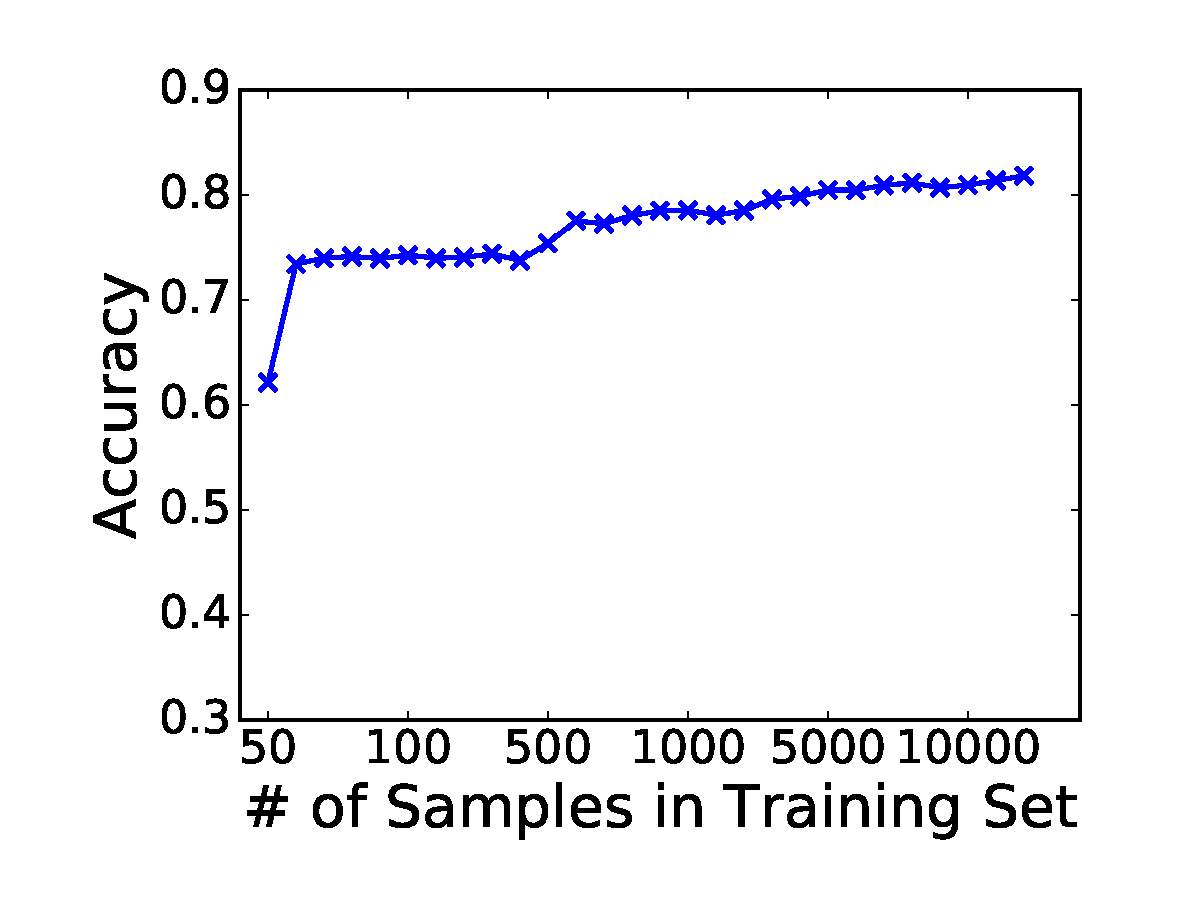
\includegraphics[width=0.16\linewidth]{figure/svm/0}\label{fig:moredata1}} 
\subfloat[Group 2]{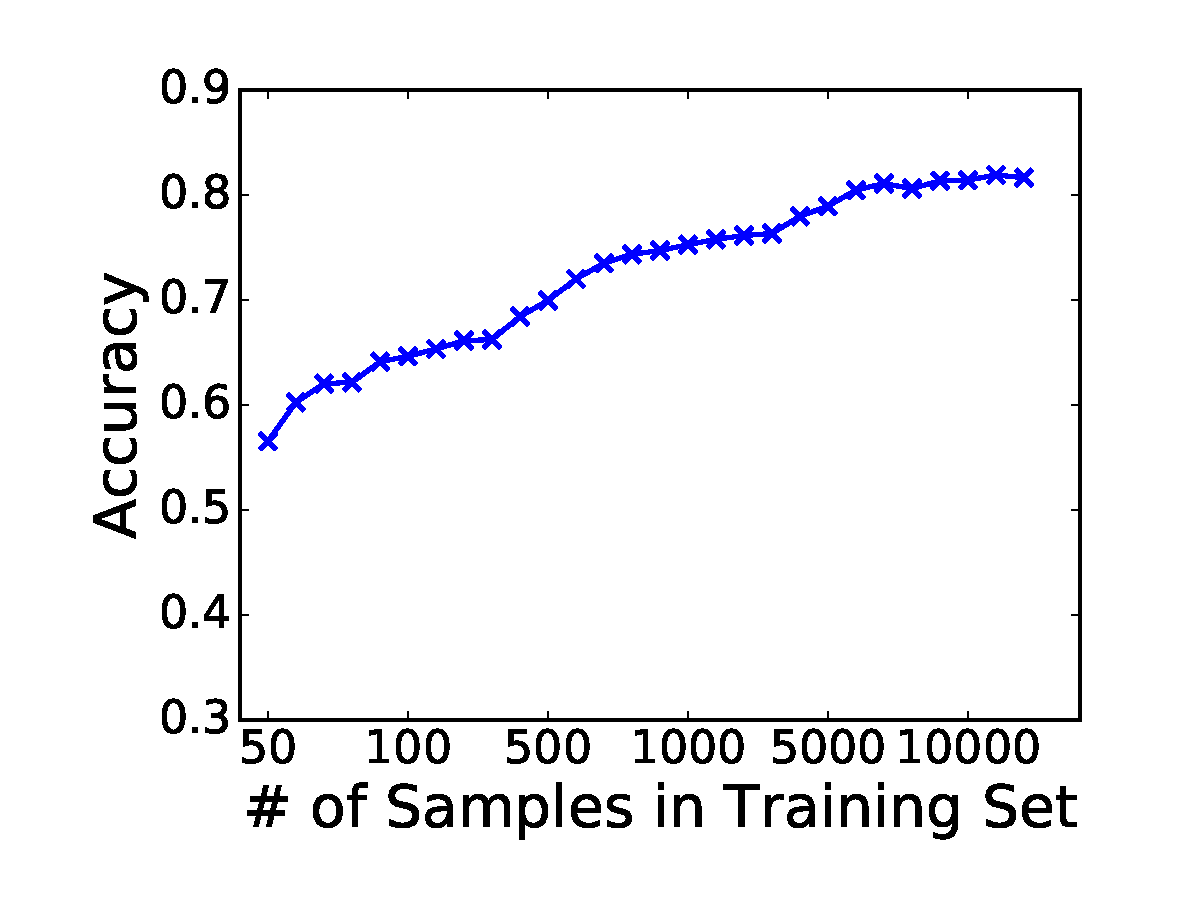
\includegraphics[width=0.16\linewidth]{figure/svm/1}\label{fig:moredata2}}
\subfloat[Group 3]{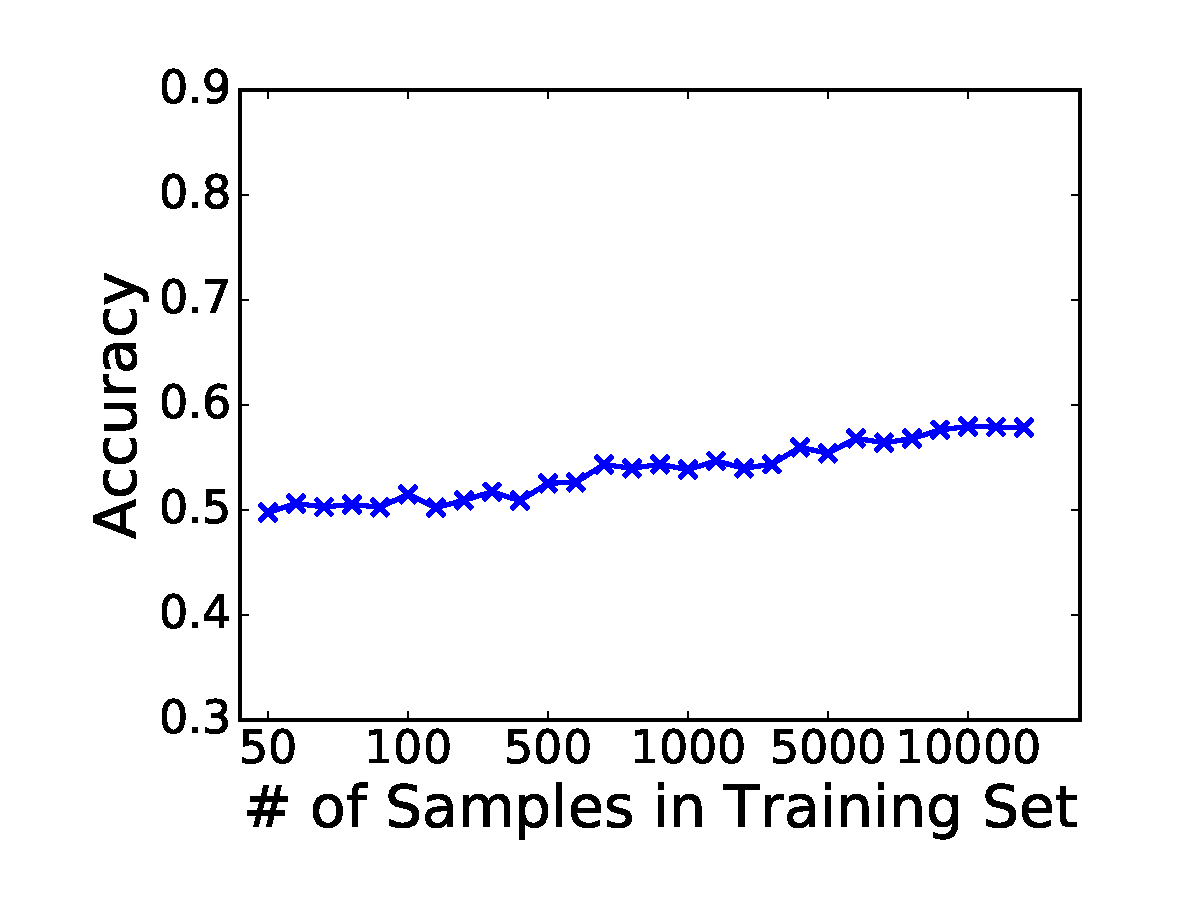
\includegraphics[width=0.16\linewidth]{figure/svm/2}\label{fig:moredata3}} 
\subfloat[Group 4]{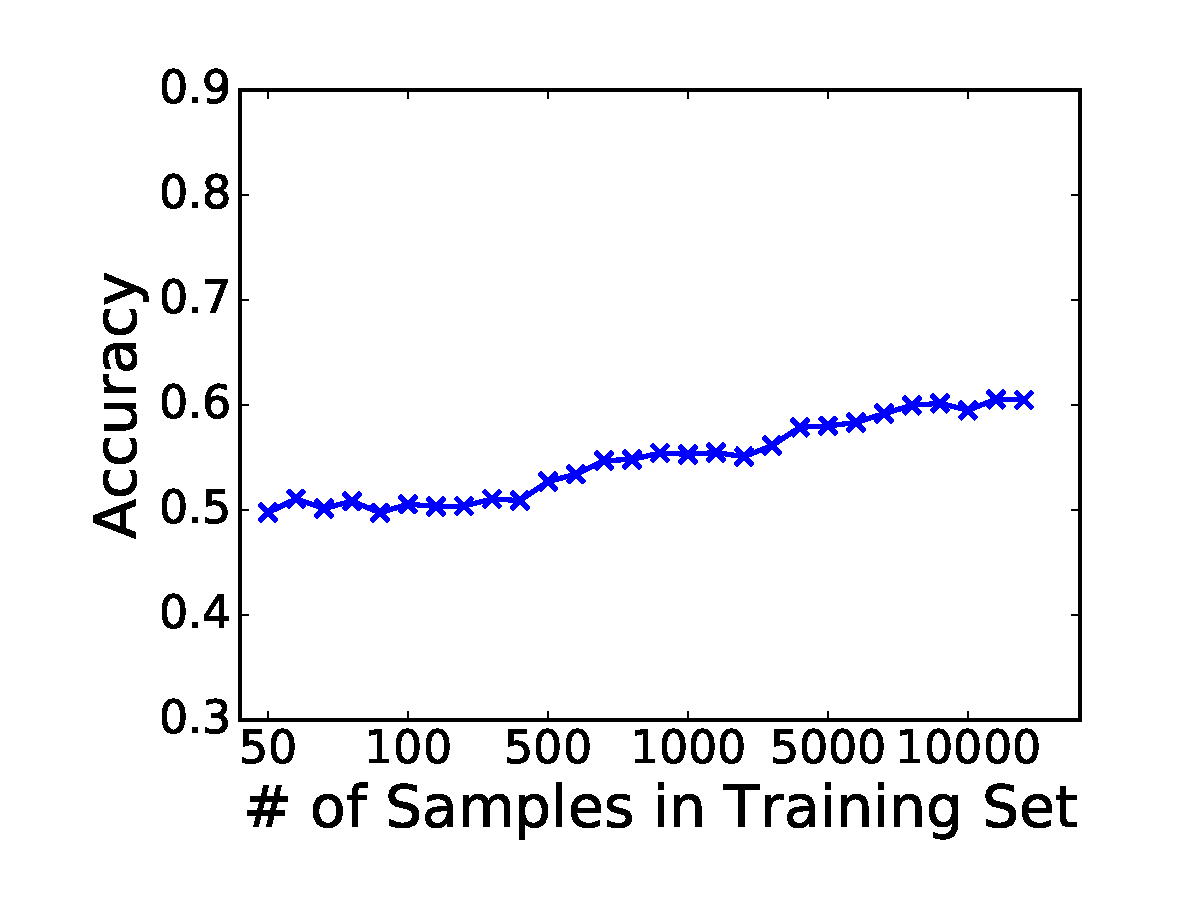
\includegraphics[width=0.16\linewidth]{figure/svm/3}\label{fig:moredata4}}
\subfloat[Group 5]{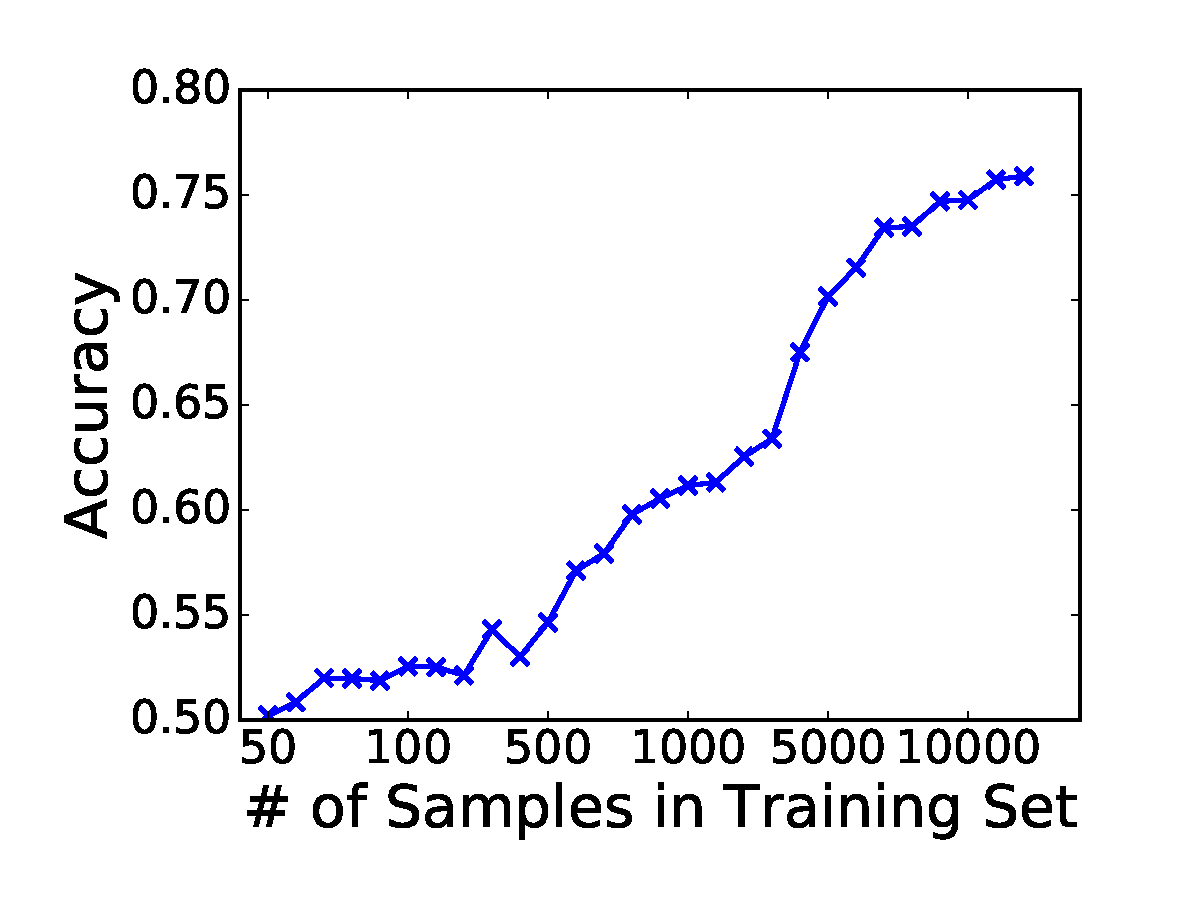
\includegraphics[width=0.16\linewidth]{figure/svm/4}\label{fig:moredata5}} \\ 

\subfloat[Group 6]{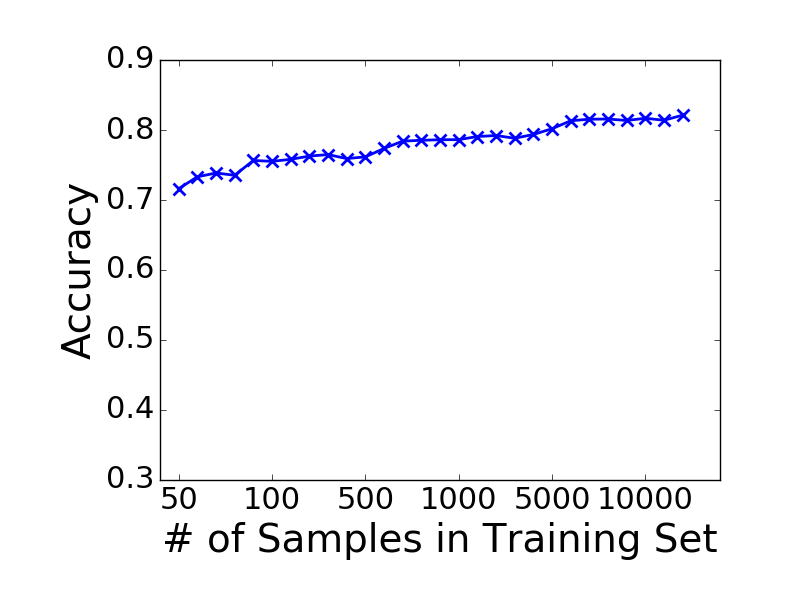
\includegraphics[width=0.16\linewidth]{figure/svm/5}\label{fig:moredata6}} 
\subfloat[Group 7]{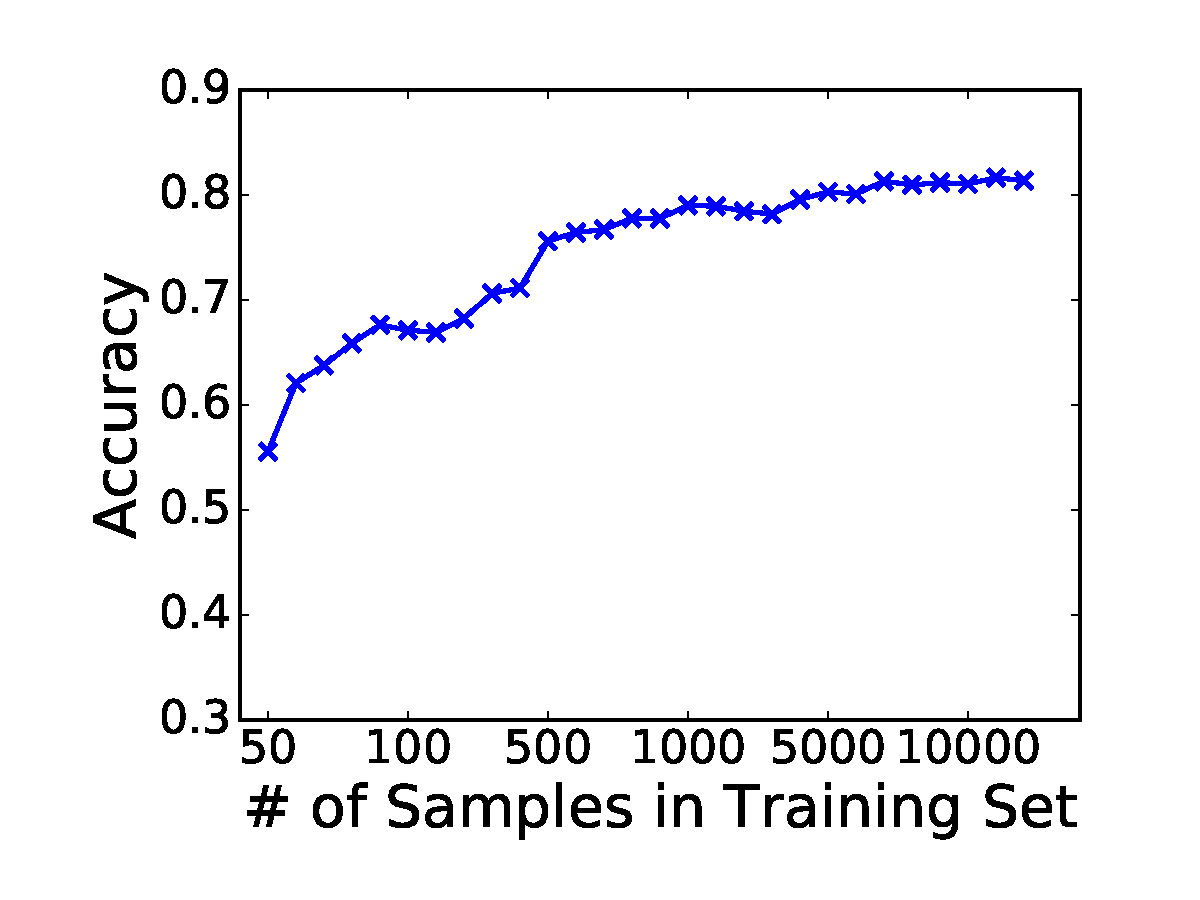
\includegraphics[width=0.16\linewidth]{figure/svm/6}\label{fig:moredata7}}
\subfloat[Group 8]{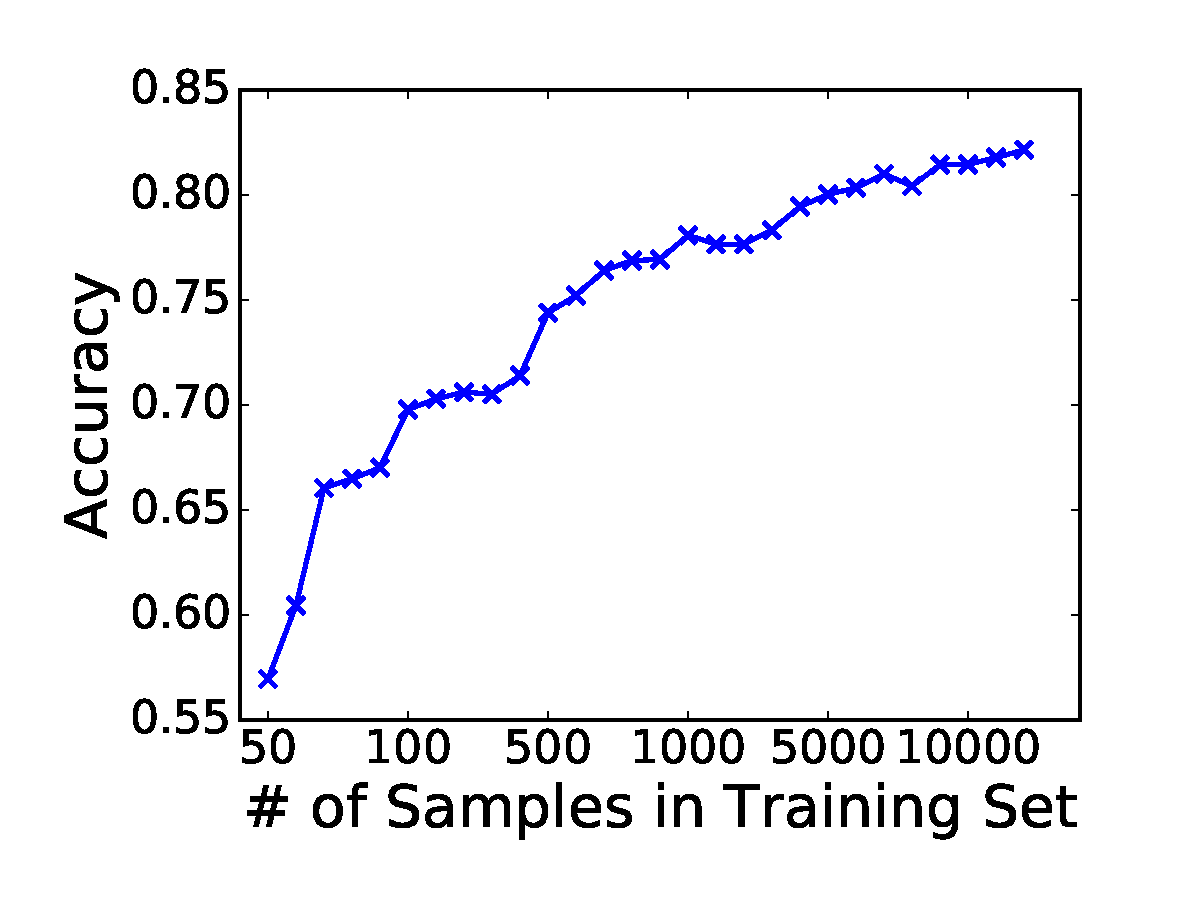
\includegraphics[width=0.16\linewidth]{figure/svm/7}\label{fig:moredata8}} 
\subfloat[Group 9]{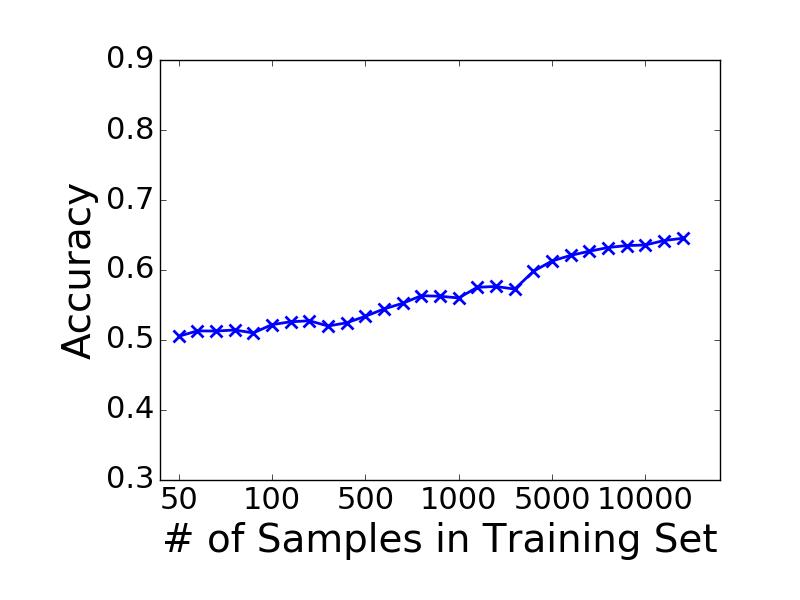
\includegraphics[width=0.16\linewidth]{figure/svm/8}\label{fig:moredata9}}
\subfloat[Group 10]{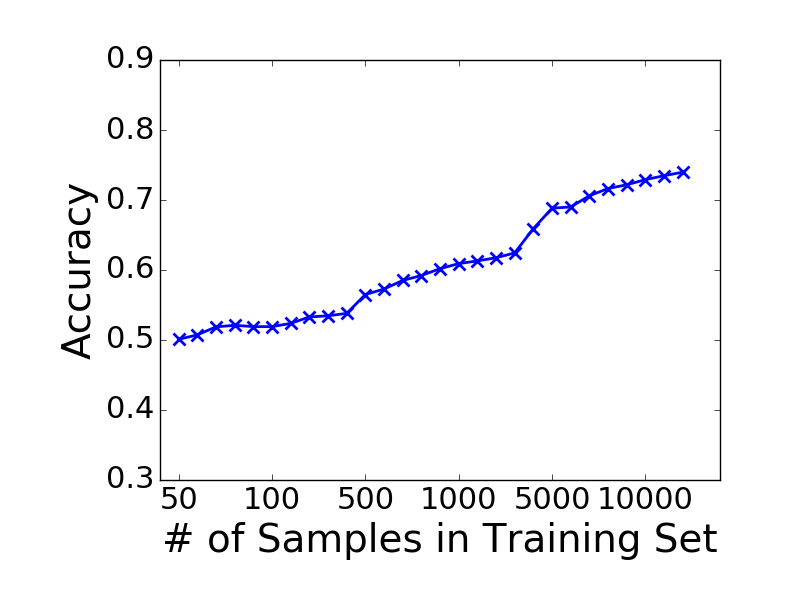
\includegraphics[width=0.16\linewidth]{figure/svm/9}\label{fig:moredata10}}
\subfloat[10-class]{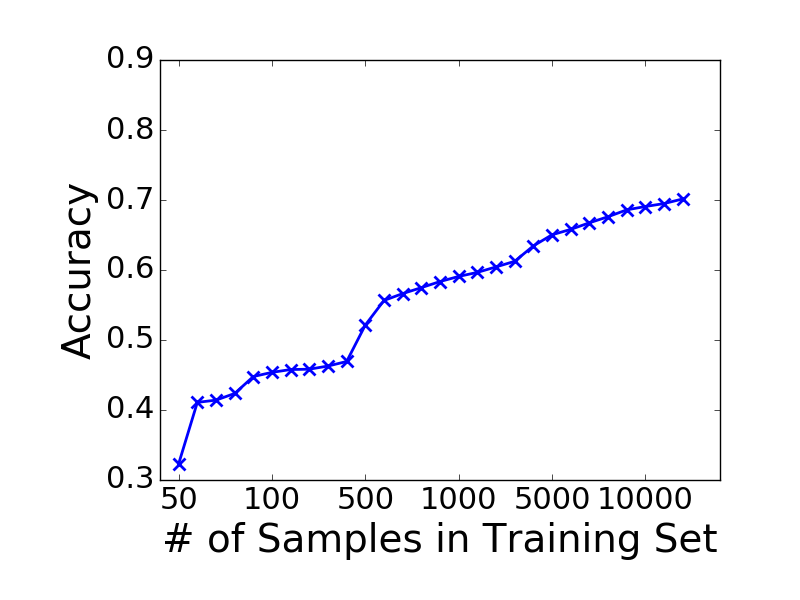
\includegraphics[width=0.16\linewidth]{figure/svm/10}\label{fig:moredata11}}
\caption{How accuracy changes with more data in traning set. 
{\footnotesize{(Figure~\ref{fig:moredata1} - Figure~\ref{fig:moredata10} show how accuracy of each two-class classifier changes 
with the size of training set changing from 50 to 10000. 
Figure~\ref{fig:moredata11} shows how accuracy of the ten-class classifier changes with the size of training set increaing from 50 to 10000. )}}} 
\label{fig:moredata} 
\end{figure*} 

\subsection{Classification Experiments}


\subsection{Discussion}
1. Future work about indexing ssdeep string
2. Upper bound
3. More data better results
4. Need human effort or dynamic information 